% Beamer template
% Author: Ozgur Taylan TURAN
% Delft University of Technology

\documentclass[aspectratio=169]{beamer}
\usepackage{/home/taylanot/texmf/tex/beamerthemetot}
% PACKAGES
\usepackage[english]{babel}
\usepackage{graphicx}
\usepackage{animate}
%\usepackage{calc}
\usepackage{calligra}
\usepackage[absolute,overlay]{textpos}
\usepackage[T1]{fontenc}
%\usefonttheme{serif}
\usefonttheme{professionalfonts}
\usepackage{amsmath}
\usepackage{palatino}
\usepackage{mathpazo}
\usepackage{graphicx}
%\usepackage{subfig}
\usepackage{tikz}
\usetikzlibrary{shapes,arrows}
\usepackage{xcolor}
\usepackage[T1]{fontenc}
%\usefonttheme{serif}
%\usepackage{titling}
\usepackage{graphicx}
%\usepackage{subfig}
%\usepackage{tikz}
%\usetikzlibrary{shapes,arrows}
\usepackage{mathtools}
\usepackage{cancel}
    
% BIB SETTINGS
\usepackage[backend=bibtex,firstinits=true,maxnames=30,maxcitenames=20,url=false,style=authoryear]{biblatex}
\bibliography{../../../Mendeley/bibtex_linux/CoffeeTalks}

\setlength\bibitemsep{0.3cm} % space between entries in the reference list
\renewcommand{\bibfont}{\normalfont\scriptsize}
\renewcommand{\cite}[1]{\footnote<.->[frame]{\fullcite{#1}}}
\setbeamertemplate{bibliography item}{}

\setbeamertemplate{navigation symbols}{} % remove navigation symbols


 % COVER PAGE INFO   
\newcommand{\mytitle}{\color{White}\huge{\textbf{Coffee Talk \#3}}}
\newcommand{\mysubtitle}{\color{Pink}\Large{\textbf{Optimal Regularization Can Mitigate Double Descent}}}
\newcommand{\myauthor}{\color{White}\textcalligra{\LARGE Ozgur Taylan Turan}}
\newcommand{\authorlabel}{\small O.T. Turan}
\author{\authorlabel}


\begin{document}
% COVER PAGE
{
{
\def\beamer@entrycode{\vspace*{-\headheight}}
\setbeamertemplate{frametitle}[default][center]
\setbeamertemplate{navigation symbols}{}
\usebackgroundtemplate{
\includegraphics[width=\paperwidth,height=\paperheight]{cover/coverart.pdf}}

\begin{frame}[plain] 

\begin{minipage}{\textwidth}
	\centering{\mytitle} \\
	%\vspace{1cm}
	%\centering{\mysubtitle} \\
	\vspace{1cm}
	\centering{\color{White}November 15, 2021} \\
	\vspace{1cm}
	\centering{\myauthor}\\
\end{minipage}
\end{frame}
}

\setbeamercovered{transparent}
\setbeamertemplate{footline}{\usebeamertemplate*{minimal footline}}
\setbeamertemplate{headline}{\usebeamertemplate*{minimal headline}}
\def\beamer@entrycode{\vspace*{-\headheight}}
}
% MAIN
\setbeamercovered{transparent}


\begin{frame}
	\centering
	\mysubtitle\cite{Nakkiran2020a}
\end{frame}

\begin{frame}{Why This Paper?}
	\centering
	\begin{minipage}{0.8\textwidth}
			\centering
			 Journey after reading Marco \& Tom's 2019 article\cite{Loog2019}
	\end{minipage}
\end{frame}

\begin{frame}{Aim}
  \centering
	\begin{minipage}{0.5\textwidth}
		\centering
      Show theoretically and empirically optimal regularization can ensure monotonicity for sample and model size under certain assumptions!
	\end{minipage}
\end{frame}

\begin{frame}{Double Descent} 
  \centering
  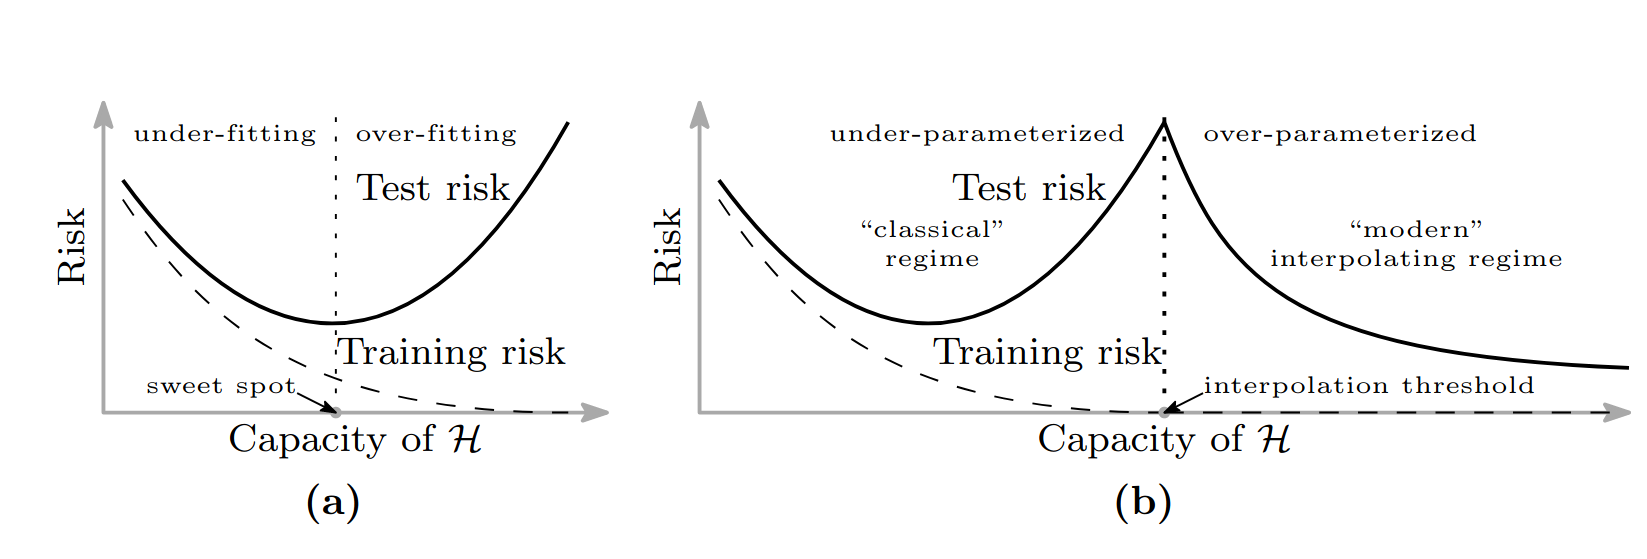
\includegraphics[width=0.8\textwidth]{Figures/doubledescent.png}\cite{Belkin2019}

  \begin{itemize}
    \item See Marco and other PR collogues work\cite{Loog2020} for a detailed history of this behaviour.
    %\item Variety of models exhibit this behaviour.
  \end{itemize}
\end{frame}

\begin{frame}{Why do we care?}

  \begin{itemize}
    \item Potential gap in understanding of generalization. (performance on new data)
    \item We want monotonic behaving models with respect to model compleixty and data.
  \end{itemize}

\end{frame}

\begin{frame}{Aim}
\color{Black}
  \centering
  \textit{When does optimally tuned regularization mitigate the double descent phenomenon?}

\vspace{3cm}

\color{Pink}{P.S.} This question implicitly assumes that double descent is observed mostly for under-regularized models.
  
\end{frame}

\begin{frame}{Remarks}

  \begin{itemize}
    \item Claims are regarding the empirical test risk.
    \item Theoretical results are derived under the assumption that the covariance of the data is isotropic.
  \end{itemize}

\end{frame}

\begin{frame}{Ridge Regression-A}

  \begin{itemize}
    \item For input $x\in\mathbb{R}^d$ generated from $\mathcal{N}(0, I_d)$ output is $y=\langle x,\beta^* \rangle + \varepsilon$ with $\varepsilon \sim \mathcal{N}(0,\sigma^2)$
    \item With the aim  to learn $f_\beta(x)=\langle x,\beta \rangle$ with n training samples drawn i.i.d. from $\mathcal{D}$ which is the joint dist. of $(x,y)$ by minimizing population mean-squared error $R(\beta):= \displaystyle\mathop{\mathbb{E}}_{(x,y)\sim\mathcal{D}}[(\langle x,\beta \rangle -y)^2]$ 
    \item with input matrix $\boldsymbol{X}\in\mathbb{R}^{n \times d}$ and output vector $\boldsymbol{y}\in\mathbb{R}^n$
    \item Ridge estimator is given by,
      \begin{align}
        \hat{\beta}_{n,\lambda} &= \displaystyle\mathop{\text{argmin}}_\beta ||\boldsymbol{X}\beta-\boldsymbol{y}||^2 + \lambda||\beta||^2 \\
      &= (\boldsymbol{X}^T\boldsymbol{X}+\lambda I_d)^{-1}\boldsymbol{X}^T\boldsymbol{y}
      \end{align}
  \end{itemize}

\end{frame}

\begin{frame}{Ridge Regression-B}
  
  \begin{itemize}
    \item  Optimal ridge parameter for n samples is given by,
      \begin{equation}
        \lambda_n^{\text{opt}} = \displaystyle\mathop{\text{argmin}}_\lambda \bar{R}(\hat{\beta}_{n,\lambda})
      \end{equation}
where, $\bar{R}(\hat{\beta}_{n,\lambda}) = \displaystyle\mathop{\mathbb{E}}_{\boldsymbol{X},\boldsymbol{y}\sim \mathcal{D}^n}[R(\hat{\beta}_n(\boldsymbol{X},\boldsymbol{y})]$
    \end{itemize}
\end{frame}

\begin{frame}{Sample Monotonicity in Ridge Reg.}

\only<1>{ \begin{itemize}
    \item<1> The expected risk of optimally regularized well-specified isotropic(/non-isotropic?) linear reg. is monotonic in samples. $\to \bar{R}(\hat{\beta}^{\text{opt}}_{n+1})\leq \bar{R}(\hat{\beta}^{\text{opt}}_{n})$
    
 \end{itemize}}

\only<2> {\centering$\displaystyle\mathop{\mathbb{E}}_{\Gamma_n}\Bigg[\sum_{i=1}^d \frac{\sigma^2}{\gamma_i^2+d\sigma^2/||\beta^*||^2}\Bigg]\leq\displaystyle\mathop{\mathbb{E}}_{\Gamma_{n+1}}\Bigg[\sum_{i=1}^d \frac{\sigma^2}{\tilde{\gamma}_i^2+d\sigma^2/||\beta^*||^2}\Bigg]$ 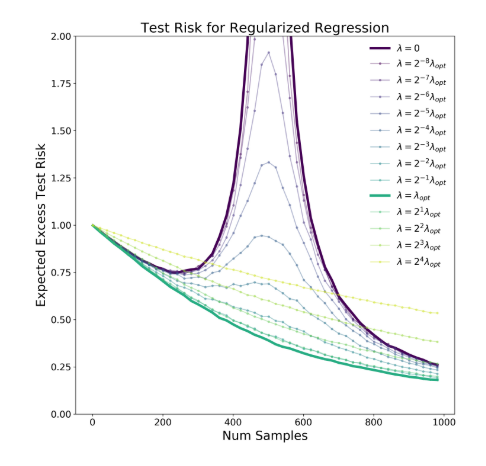
\includegraphics[width=0.4\textwidth]{Figures/ex1.png}}

\only<1> {Closed form solution? So, ...}
\begin{block}{\color{White} The Basic Idea}
Noting that all the notation with $\sim$ on correspond to $n+1$ samples and the rest belongs to $n$ samples.
\begin{itemize}
  \item <1> Let $\gamma$ be the singular values of $\boldsymbol{X}\in\mathbb{R}^{n\times d}$ which are distributed with $\Gamma_n$.
  \item <1> Isotropy of $x$ and exploiting interlacing between $\Gamma_n$ and $\Gamma_{n+1}$ allows, $\bar{R}(\hat{\beta}_{n}^{\text{opt}})=\displaystyle\mathop{\mathbb{E}}_{\Gamma_n}\Bigg[\sum_{i=1}^d \frac{\sigma^2}{\gamma_i^2+d\sigma^2/||\beta^*||^2}\Bigg]+\sigma^2$. Noting that interlacing ensures $\gamma_i\leq \tilde{\gamma}_i$
\end{itemize} 
\end{block}

\end{frame}

\begin{frame}{Model Monotonicity Ridge Reg.}
\begin{block}{\color{White}Remark}
\begin{itemize}
  \item Only for this section it is assumed that the covariates live in $p$-dimensional space, but the regression model is employed after projection to a $d$-dimensional space $(\boldsymbol{X}\in\mathbb{R}^{n\times p})$. Then, $\tilde{\boldsymbol{X}}\boldsymbol{P}^T$ where $\boldsymbol{P}\in\mathbb{R}^{d\times p}$ is a random orthonormal matrix.
\end{itemize}
\end{block}

\begin{itemize}
  \item Risk of the estimator $\bar{R}(\hat{\beta}) = \displaystyle\mathop{\mathbb{E}}_{\boldsymbol{P}}\mathop{\mathbb{E}}_{\tilde{\boldsymbol{X}},\boldsymbol{y}\sim \mathcal{D}^n}[R_P(\hat{\beta}_n(\tilde{\boldsymbol{X}},\boldsymbol{y}))]$
  \item In similar fashion $\bar{R}(\hat{\beta}^{\text{opt}}_{d+1})\leq \bar{R}(\hat{\beta}^{\text{opt}}_{d})$
\end{itemize}

\end{frame}

\begin{frame}
  Similar emprical results on Random ReLU Features and CNN's.
\end{frame}

\begin{frame}{Conclusions}
\begin{itemize}
  \item Certain linear models optimal $\ell2$ regularization can prevent non-monotonic behaviour.
  \item Investigation of more complicated and nonlinear models?
\end{itemize}
  
\end{frame}
\end{document}

